% The last scattering surface: a photon random-walks through the ionised
% plasma, scattering off free electrons, until recombination binds them into
% neutral hydrogen; after its last scattering it streams freely to us.
% Simplified redraw of Yacine Ali-Haimoud's sketch (NYU, 2019), on the slide palette.
% Compile: pdflatex last_scattering.tex && pdftocairo -svg last_scattering.pdf last_scattering.svg
\documentclass[tikz,border=4pt]{standalone}
\usepackage{tikz}
\usepackage[T1]{fontenc}
\usetikzlibrary{arrows.meta,decorations.pathmorphing,calc}

\definecolor{ink}{HTML}{2E2E2E}
\definecolor{greytx}{HTML}{6E6E6E}
\definecolor{ecol}{HTML}{C2560A}   % electrons
\definecolor{pcol}{HTML}{3B6FB6}   % protons
\definecolor{hcol}{HTML}{521463}   % neutral hydrogen
\definecolor{phot}{HTML}{E0A21B}   % photon
\definecolor{warm}{HTML}{F7DCCB}
\definecolor{cool}{HTML}{D3E3F4}

\def\W{16}     % band width
\def\H{4.6}    % band height
\def\ls{9.2}   % last scattering, centre of the shaded strip

\tikzset{
  photon/.style={phot,line width=1.8pt,line cap=round,
    decorate,decoration={snake,amplitude=0.9mm,segment length=2.6mm,post length=2.4mm}},
}
\newcommand{\elec}[1]{\fill[ecol] #1 circle (0.09);}
\newcommand{\prot}[1]{\fill[pcol] #1 circle (0.17);}
\newcommand{\hyd}[1]{%
  \begin{scope}[shift={(#1)}]
    \draw[hcol,line width=1.2pt] (0,0) ellipse (0.36 and 0.24);
    \fill[pcol] (-0.09,0) circle (0.13);
    \fill[ecol] (0.17,0.05) circle (0.07);
  \end{scope}}

\begin{document}
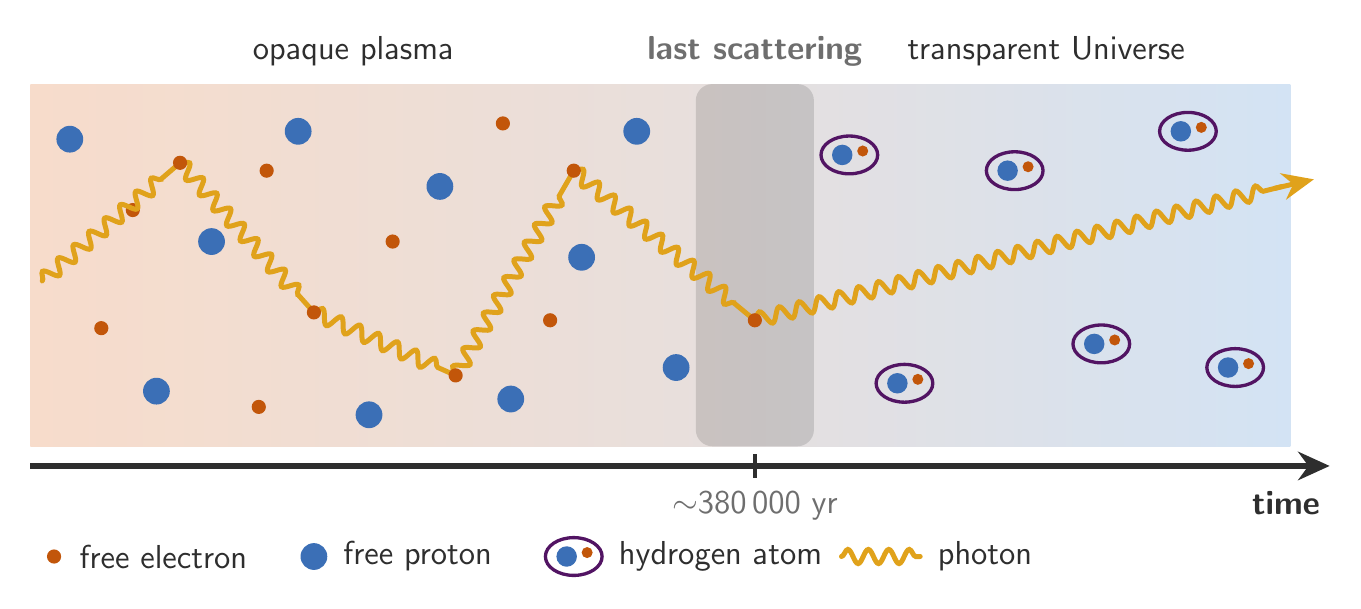
\begin{tikzpicture}[font=\sffamily]

% ---------------------------------------------------------------- band
\shade[left color=warm,right color=cool,middle color=cool!40!warm]
      (0,0) rectangle (\W,\H);
\fill[ink,opacity=0.16,rounded corners=6pt] (\ls-0.75,0) rectangle (\ls+0.75,\H);

% ---------------------------------------------------------------- plasma: free protons and electrons
\foreach \p in {(0.5,3.9),(1.6,0.7),(2.3,2.6),(3.4,4.0),(4.3,0.4),
                (5.2,3.3),(6.1,0.6),(7.0,2.4),(7.7,4.0),(8.2,1.0)}
  {\prot{\p}}
\foreach \p in {(0.9,1.5),(1.3,3.0),(2.9,0.5),(3.0,3.5),(4.6,2.6),
                (6.0,4.1),(6.6,1.6)}
  {\elec{\p}}

% ---------------------------------------------------------------- after recombination: neutral hydrogen
\foreach \x/\y in {10.4/3.7,11.1/0.8,12.5/3.5,13.6/1.3,14.7/4.0,15.3/1.0}
  {\hyd{\x,\y}}

% ---------------------------------------------------------------- photon: random walk, then free streaming
\coordinate (a0) at (0.15,2.1);
\coordinate (a1) at (1.9,3.6);
\coordinate (a2) at (3.6,1.7);
\coordinate (a3) at (5.4,0.9);
\coordinate (a4) at (6.9,3.5);
\coordinate (a5) at (\ls,1.6);    % last scattering
\coordinate (a6) at (\W-0.1,3.3);
\foreach \i/\j in {a0/a1,a1/a2,a2/a3,a3/a4,a4/a5} {\draw[photon] (\i) -- (\j);}
\draw[photon] (a5) -- (a6);
\draw[phot,-{Stealth[length=4mm,width=3.4mm]},line width=1.8pt] ($(a5)!0.985!(a6)$) -- ($(a6)+(0.4,0.09)$);
\foreach \c in {a1,a2,a3,a4,a5} {\elec{(\c)}}

% ---------------------------------------------------------------- labels
\node[greytx,font=\sffamily\bfseries\large,anchor=south] at (\ls,\H+0.1) {last scattering};
\node[ink,font=\sffamily\large,anchor=south] at (\ls/2-0.5,\H+0.1) {opaque plasma};
\node[ink,font=\sffamily\large,anchor=south] at (12.9,\H+0.1) {transparent Universe};

% ---------------------------------------------------------------- time axis
\draw[ink,line width=2pt,-{Stealth[length=4mm,width=3.6mm]}] (0,-0.25) -- (\W+0.5,-0.25);
\draw[ink,line width=1.2pt] (\ls,-0.1) -- (\ls,-0.4);
\node[greytx,font=\sffamily\large,anchor=north] at (\ls,-0.45) {$\sim$380\,000 yr};
\node[ink,font=\sffamily\bfseries\large,anchor=north east] at (\W+0.5,-0.45) {time};

% ---------------------------------------------------------------- legend
\begin{scope}[shift={(0.3,-1.4)},font=\sffamily\large]
  \fill[ecol] (0,0) circle (0.09);
  \node[ink,anchor=west] at (0.2,0) {free electron};
  \fill[pcol] (3.3,0) circle (0.17);
  \node[ink,anchor=west] at (3.55,0) {free proton};
  \hyd{6.6,0}
  \node[ink,anchor=west] at (7.05,0) {hydrogen atom};
  \draw[photon,decoration={post length=0mm}] (10.0,0) -- (11.0,0);
  \node[ink,anchor=west] at (11.1,0) {photon};
\end{scope}

\end{tikzpicture}
\end{document}
